\begin{problem}
Determinar os três vértices de um triângulo sabendo que os pontos médios de seus lados são
$$M = (5,0,-2), \ N=(3,1,-3)\ \text{e}\ P=(4,2,1).$$
\end{problem}

\begin{solution}A figura a seguir fixa a notação utilizada e também ajuda a entender a solução.

\centerline{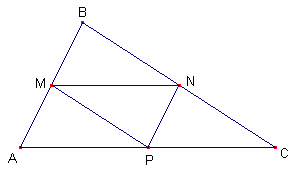
\includegraphics[scale=0.6]{img/bank_vetores/fig03.png}}

Sabemos que segmentos orientados paralelos, com o mesmo comprimento e com o mesmo sentido representam o mesmo vetor. Além disso, como o segmento que une os pontos médios de dois lados de um triângulo é paralelo e tem a metade do comprimento do terceiro lado vemos, por exemplo, que
$\overrightarrow{AP} = \overrightarrow{MN}$, $\overrightarrow{PC} = \overrightarrow{MN}$ e $\overrightarrow{MB} = \overrightarrow{PN}$. Daí 

\begin{itemize}
\item $\overrightarrow{AP}=\overrightarrow{MN}\ \Rightarrow\ P-A=N-M\ \Rightarrow\ A=M-N+P\ \Rightarrow\ A=(6,1,2)$.

\item $\overrightarrow{MB}=\overrightarrow{PN}\ \Rightarrow\ B-M=N-P\ \Rightarrow\ B=M+N-P\ \Rightarrow\ B=(4,-1,-6)$.

\item $\overrightarrow{PC}=\overrightarrow{MN}\ \Rightarrow\ C-P=N-M\ \Rightarrow\ C=-M+N+P\ \Rightarrow\ C=(2,3,0)$.
\end{itemize}

Portanto os vértices do triângulo são os pontos $(6,1,2)$, $(4,-1,-6)$ e $(2,3,0)$. 
\end{solution}


\begin{problem}
Sendo $A=(2,-5,3)$ e $B=(7,3,-1)$ vértices consecutivos de um \linebreak 
paralelogramo $ABCD$ e $M=(4,-3,3)$ o ponto de interseção das diagonais, determine os vértices $C$ e $D$.
\end{problem}

\begin{solution}
Observe a figura a seguir.

\centerline{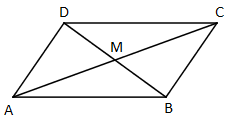
\includegraphics[scale=0.8]{img/bank_vetores/fig04.png}}

\begin{itemize}
\item $\overrightarrow{MC}=\overrightarrow{AM}\ \Rightarrow\ C-M=M-A\ \Rightarrow\ C=2M-A\ \Rightarrow\ C=(6,-1,3)$.

\item $\overrightarrow{MD}=\overrightarrow{BM}\ \Rightarrow\ D-M=M-B\ \Rightarrow\ D=2M-B\ \Rightarrow\ D=(1,-9,7)$. 
\end{itemize}
\end{solution} 






\begin{problem} 
Em um plano cartesiano considere os pontos $A=(4,6)$ e $B=(6,5)$. Determine um ponto $C$ sobre o eixo $x$ e determine um ponto $D$ no eixo $y$ de modo que $ABCD$ seja um paralelogramo contido no primeiro quadrante.
\end{problem}

\begin{solution}
Observe a figura a seguir.

\centerline{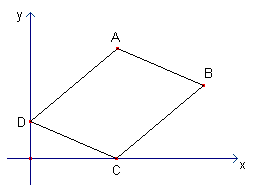
\includegraphics[scale=0.6]{img/bank_vetores/fig05.png}}

O ponto $C=(x,0)$ e o ponto $D=(0,y)$ são tais que $\overrightarrow{DC}=\overrightarrow{AB}$. Daí $C-D=B-A$ $\Rightarrow$ $(x,0)-(0,y)=(2,-1)$ 
$\Rightarrow$ $(x,-y)=(2,-1)$ $\Rightarrow$ $x=2$ e $y=1$. Portanto $C=(2,0)$ e $D=(0,1)$. 
\end{solution}


\begin{problem}
Em um plano cartesiano está desenhado o quadrado $ABCD$ tal que $A=(1,2)$ e $B=(6,5)$.
Determine as coordenadas dos vértices $C$ e $D$.

\centerline{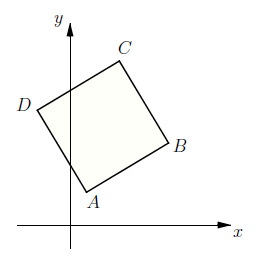
\includegraphics[scale=0.8]{img/bank_vetores/fig12.png}}

\end{problem}


\begin{solution} 
Temos que $\overrightarrow{AB}=B-A=(5,3)$.
Como o vetor $\overrightarrow{AD}$ é obtido por uma rotação de $90^o$ no sentido anti-horário do vetor $\overrightarrow{AB}$ segue que

$$\overrightarrow{AD}\ =\ R_{90^0} \left(\overrightarrow{AD}\right)\ =\ 
\left[\begin{array}{rr} 0 & -1 \\ 1 & 0 \end{array}\right]\,
\left[\begin{array}{r} 5 \\ 3 \end{array}\right]\ =\ 
\left[\begin{array}{r} -3 \\ 5 \end{array}\right]$$

Assim vemos que $\overrightarrow{AD}=(-3,5)$. Como $\overrightarrow{AD}=D-A$, segue que 
$$D = A + \overrightarrow{AD} = (1,2) + (-3,5) = (-2,7)$$

\medskip
Pela regra do paralelogramo, temos que $\overrightarrow{AC} = \overrightarrow{AB} + \overrightarrow{AD}$.
Daí segue que $C-A = (B-A) + (D-A)$ e portanto
$$C = B + D - A = (6,5) + (-2,7) - (1,2) = (3,10)$$  

\end{solution}

\begin{problem} 
Determine as coordenadas do ponto $P$ que está no eixo $x$ e que é \linebreak
equidistante dos pontos $A=(3,-1,4)$ e $B=(1,-2,-3)$.
\end{problem}

\begin{solution}
Queremos um ponto $P=(x,0,0)$ tal que $\dist(P,A)=\dist(P,B)$. Como distância é um número positivo, esta igualdade é equivalente a
$\dist^2(P,A)=\dist^2(P,B)$.
  
$$\dist(P,A)^2 = (x-3)^2 + 1 + 16 \ \ \ \ \ \ \ \ \ \ \ \dist(P,B)^2 = (x-1)^2 + 4 + 9.$$

\medskip
Daí $\dist(P,A)^2=\dist(P,B)^2$ implica $(x-3)^2 + 1 + 16=(x-1)^2 + 4 + 9$ cuja solução é $x=3$. Portanto $P=(3,0,0).$ 
\end{solution}




\begin{problem}
Responda as seguintes questões sobre vetores em um plano cartesiano.
\begin{enumerate}
\item[(a)] Dados dois vetores $V$ e $W$, sabemos que a soma $V+W$ pode ser obtida pela regra do paralelogramo. O vetor $V+W$ é um vetor que está na direção da reta bissetriz do ângulo formado por $V$ e $W$? Em outras palavras, a diagonal $V+W$ do paralelogramo divide os ângulos deste paralelogramo em dois ângulos iguais? 

\item[(b)] Qual é a condição sobre $V$ e $W$ para que a resposta do item (a) seja afirmativa?

\item[(c)] No plano cartesiano considere os vetores $V=(3,4)$ e $W=(12,5)$. Determine um vetor que está na direção da reta bissetriz do ângulo formado por $V$ e $W$.
\end{enumerate}
\end{problem}

\begin{solution} 
\begin{enumerate}
\item[(a)] A figura a seguir mostra que, em geral, o vetor $V+W$ não está na direção da bissetriz do ângulo formado pelos vetores $V$ e $W$. Observe que nesta figura $\alpha \neq \beta$.

\centerline{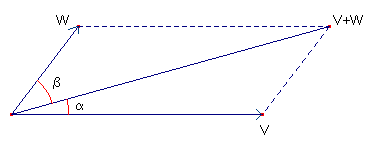
\includegraphics[scale=0.6]{img/bank_vetores/fig06.png}}

\item[(b)] Se $V$ e $W$ tiverem a mesma norma, então o paralelogramo de lados paralelos a $V$ e a $W$ é, de fato, um losango. Neste caso, as diagonais do losango estão nas direções das bissetrizes dos ângulos internos do losango.

\item[(c)] Se $V=(3,4)$ e se $W=(12,5)$ então $\hmod{V}=\sqrt{9+16}=5$ e $\hmod{W}=\sqrt{144+25}=13$. Como estes vetores não possuem a mesma norma, vimos que o vetor $V+W$ não está na direção da reta bissetriz do ângulo entre $V$ e $W$. Para determinar esta bissetriz podemos multiplicar $V$ por um número $a$ e podemos multiplicar $W$ por um número $b$ de modo que os vetores $aV$ e $bW$ possuem a mesma norma. Daí, como vimos no item anterior, o vetor $aV+bW$ está na direção da reta bissetriz. (veja figura a seguir)

\centerline{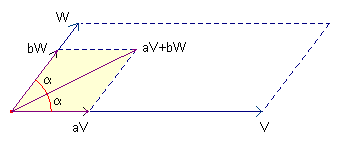
\includegraphics[scale=0.6]{img/bank_vetores/fig07.png}}

Existem várias escolhas para estes escalares $a$ e $b$. Existem alunos que preferem dividir $V$ e $W$ pelas suas normas, para obter vetores unitários. Outra possibilidade, para evitar frações, é multiplicar cruzado: $V$ pela norma de $W$ e multiplicar $W$ pela norma de $V$. Fazendo isso no nosso exemplo, obtemos os vetores $13V=(39,52)$ e $5W=(60,25)$. Estes dois vetores possuem norma $5\times 13 = 65$ e são tais que a soma
$13V+5W=(99, 77)$ é um vetor na direção da reta bissetriz do ângulo entre $V$ e $W$. 

Observe que qualquer múltiplo deste vetor também é um outro vetor na direção da reta bissetriz do ângulo entre $V$ e $W$. Assim, multiplicando este vetor $13V+5W=(99, 77)$ por $\dfrac{1}{11}$ encontramos o vetor $(9,7)$ que também está na direção da reta bissetriz do ângulo entre $V$ e $W$. 
\end{enumerate}
\end{solution}

\begin{problem}
Em um plano cartesiano, determine a equação da reta bissetriz do menor ângulo formado pelo eixo $x$ e pela reta de equação $y=2x$.
\end{problem}

\begin{solution}
Vamos utilizar o resultado da questão anterior. Observe que o vetor \linebreak
$V=(1,0)$ aponta na direção do eixo $x$.
Por outro lado, o vetor $W=(1,2)$ aponta na direção da reta $y=2x$.
As normas desses vetores são $||V||=1$ e $||W||=\sqrt{5}$.
Daí os vetores $\sqrt{5}\, V = \left(\sqrt{5}\ ,0\right)$ e $1\, W = (1,2)$ possuem a mesma norma.
Como discutido na questão anterior, temos que o vetor
$$\sqrt{5}\, V + 1\, W = \left(1 + \sqrt{5}\ , 2\right)$$ 
aponta na direção da reta bissetriz desejada.
A inclinação dessa reta é 
$$\dfrac{\Delta y}{\Delta x} = \dfrac{2}{1+\sqrt{5}} = \dfrac{-1 + \sqrt{5}}{2}$$
A equação da reta bissetriz desejada é
$$y =  \dfrac{-1 + \sqrt{5}}{2} x$$

\end{solution}


\begin{problem}
O vetor $V$ é ortogonal aos vetores $U=(1,2,0)$ e $W=(2,0,1)$ e forma ângulo agudo com o vetor $\vec{j}=(0,1,0)$. Determine $V$ sabendo que
$\hmod{V} = \sqrt{21}$.
\end{problem}

\begin{solution}
Estamos procurando um vetor $V=(x,y,z)$ tal que $\herm{V,U}=0$ e $\herm{V,W}=0$. Estas duas equações definem o seguinte sistema linear homogêneo

$$\left\{ \begin{array}{ccc} x+2y & = & 0 \\ 2x+z & = & 0 \end{array} \right.$$

Considerando $x$ como variável livre, podemos escrever $y=-\dfrac{x}{2}$ e $z=-2x$. Daí, por enquanto, podemos concluir que $V$ tem a forma

$$V = \left(  x, -\dfrac{x}{2} , -2x \right) .$$   

\medskip
Como $\hmod{V}=\sqrt{21}$, obtemos $\sqrt{x^2 + \dfrac{x^2}{4} + 4x^2} = \sqrt{21}$, cuja solução é $x=2$ e $x=-2$. Agora vamos analisar cada uma destas possibilidades, lembrando que para $V$ formar ângulo agudo com o vetor $\vec{j}=(0,1,0)$ é necessário que o produto escalar $\herm{V,\vec{j}}$ seja positivo.

\begin{itemize}
\item Se $x=2$ então $V = \left( 2 , -1 , -4 \right)$. Neste caso, $\herm{V,\vec{j}}=-1$ é negativo e, portanto, $x=2$ não nos interessa.

\item Se $x=-2$ então $V = \left( -2 , 1 , 4 \right)$. Neste caso, $\herm{V,\vec{j}}=1$ é positivo. Portanto obtemos como única solução deste problema o vetor $V = \left( -2 , 1 , 4 \right)$. 
\end{itemize}
\end{solution}


\begin{problem} 
Dados os pontos $A=(m,1,0)$, $B=(m-1,2m,2)$ e $C=(1,3,-1)$, detemine $m$ de modo que o triângulo $ABC$ seja retângulo em $A$. Em seguida calcule a área deste triângulo.
\end{problem}

\begin{solution}
Para o triângulo $ABC$ ser retângulo em $A$, os vetores $\overrightarrow{AB}=(-1,2m-1,2)$ e $\overrightarrow{AC}=(1-m,2,-1)$ devem ser ortogonais, ou seja, $\herm{\overrightarrow{AB},\overrightarrow{AC}}=0$. Esta equação é $-(1-m)+2(2m-1)-2=0$, cuja solução é $m=1$.

\medskip
Para $m=1$, $\overrightarrow{AB}=(-1,1,2)$ e $\overrightarrow{AC}=(0,2,-1)$. A área do triângulo pode ser calculada pela expressão: metade da base vezes a altura.

$$\text{área}(\Delta ABC)\ =\ \dfrac{\hmod{\overrightarrow{AB}}\ \hmod{\overrightarrow{AC}}}{2}\ =\ \dfrac{\sqrt{6}\ \sqrt{5}}{2}\ =\ \dfrac{\sqrt{30}}{2}. $$  
\end{solution}


\begin{problem}
Em um plano cartesiano, sejam $A=(0,0)$ e $B=(2,1)$. Determine o ponto $C$ deste plano de modo que o triângulo $ABC$ seja retângulo em $A$ e tenha ângulo de $30^o$ no vértice $B$.
\end{problem}

\begin{solution}
Queremos um ponto $C=(x,y)$ tal que os vetores $\overrightarrow{AB}=(2,1)$ e $\overrightarrow{AC}=(x,y)$ sejam ortogonais. Isto significa que $2x+y=0$. Logo $y=-2x$ e $C$ tem a forma $C=(x,-2x)$ para algum número real $x$.

\medskip
Também queremos que o ângulo entre os vetores $\overrightarrow{BC}=(x-2,-2x-1)$ e $\overrightarrow{BA}=(-2,-1)$ seja igual a $30^o$. Utilizando a expressão 

$$\cos(30^o) = \frac{\herm{ \overrightarrow{BC}\ ,\ \overrightarrow{BA}} }{ \hmod{\overrightarrow{BC}}\ \hmod{\overrightarrow{BA}}}$$

obtemos a igualdade

$$\dfrac{-2(x-2) -(-2x-1)}{\ \sqrt{(x-2)^2 + (-2x-1)^2}\ \ \sqrt{5}\ }\ =\ \dfrac{\sqrt{3}}{2}.$$

Simplificando e elevando ao quadrado obtemos $3x^2-1=0$, cujas soluções são $x=\dfrac{\sqrt{3}}{3}$ e $x=-\dfrac{\sqrt{3}}{3}$. Portanto obtemos duas soluções para este problema:

\medskip

$$C=\left(\frac{\sqrt{3}}{3} ,-\frac{2\sqrt{3}}{3}\right)\ \ \ \ \ \text{e}\ \ \ \ \ 
  C=\left(-\frac{\sqrt{3}}{3}, \frac{2\sqrt{3}}{3}\right) .$$

\centerline{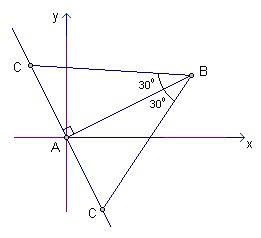
\includegraphics[scale=0.6]{img/bank_vetores/fig08.png}}

\end{solution}





\begin{problem} 
Em um plano cartesiano, considere $A=(2,1)$ e $B=(-3,4)$. Determine todos os pontos $P$ sobre o eixo $x$ tal que o triângulo
$ABP$ é retângulo no vértice $P$.
\end{problem}

\begin{solution}
Um ponto $P$ sobre o eixo $x$ pode ser escrito como $P=(x,0)$
Para o triângulo $ABP$ ser retângulo no vértice $P$, os vetores 
$\overrightarrow{PA}=A-P=(2-x,1)$ e  $\overrightarrow{PB}=B-P=(-3-x,4)$ devem ser ortogonais. 
Isso ocorre somente quando o produto escalar entre esses vetores é igual a zero. Nesse caso temos
$$\left<\overrightarrow{PA},\ \overrightarrow{PB}\right> = (2-x)(-3-x) + 4 = x^2 + x - 2$$
Resolvendo a equação $x^2+x-2=0$ obtemos $x=-2$ e $x=1$. Portanto obtemos dois pontos:
$$P_1=(-2,0)\ \ \ \text{e} \ \ \ P_2=(1,0)$$

\pagebreak
Observação. Essa questão pode ser interpretada geometricamente do seguinte modo.
Se $ABP$ é um triângulo retângulo no vértice $P$, então $P$ está sobre a circunferência de diâmetro $AB$.
Portanto, os dois pontos encontrados na solução dessa questão são os pontos de interseção do eixo $x$ com essa circunferência.


\centerline{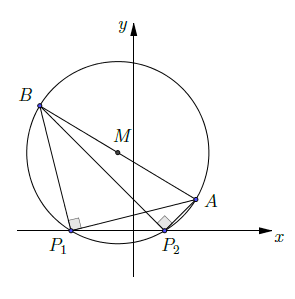
\includegraphics[scale=0.8]{img/bank_vetores/fig13.png}}
\end{solution}

\begin{problem}
Utilize o produto escalar para mostrar que 
$$A=(-1,1,2)\ ,\ \  B=(-2,8,5)\ \  \text{e}\ \ C=(-4,3,1)$$
são vértices de um triângulo retângulo. Em seguida calcule a área desse triângulo.
\end{problem}

\begin{solution}O ângulo no vértice $A$ é reto se os vetores  $\overrightarrow{AB}=B-A=(-1,7,3)$ e  $\overrightarrow{AC}=C-A=(-3,2,-1)$ são ortogonais. Isso ocorre somente quando o produto escalar entre esses vetores é igual a zero. Nesse caso temos

$$\left<\overrightarrow{AB}, \overrightarrow{AC}\right> = 3 + 14 - 3 = 14$$

Como esse número é positivo, o ângulo no vértice $A$ é agudo, menor que $90^o$.

Agora vamos verificar se o ângulo no vértice $B$ é reto.
Esse é o caso se os vetores  $\overrightarrow{BA}=A-B=(1,-7,-3)$ e  $\overrightarrow{BC}=C-B=(-2,-5,-4)$ são ortogonais. Isso ocorre somente quando o produto escalar entre esses vetores é igual a zero. Nesse caso temos

$$\left<\overrightarrow{BA}, \overrightarrow{BC}\right> = -2 + 35 + 12 = 45$$

Como esse número é positivo, o ângulo no vértice $B$ é agudo, menor que $90^o$.


Agora vamos verificar se o ângulo no vértice $C$ é reto.
Esse é o caso se os vetores  $\overrightarrow{CA}=A-C=(3,-2,1)$ e  $\overrightarrow{CB}=B-C=(2,5,4)$ são ortogonais. Isso ocorre somente quando o produto escalar entre esses vetores é igual a zero. Nesse caso temos

$$\left<\overrightarrow{CA}, \overrightarrow{CB}\right> = 6 - 10 + 4 = 0$$

Como esse produto escalar é igual a zero, concluímos que o triângulo $ABC$ é retângulo no vértice $C$.

\centerline{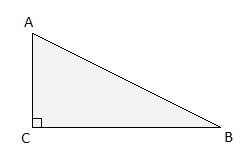
\includegraphics[]{img/bank_vetores/fig11.png}}

Podemos calcular a área de um triângulo pela fórmula šbase vezes altura dividido por dois''. No caso de um triângulo retângulo, podemos considerar um cateto como base e o outro cateto como altura. Daí, no nosso caso, a área pode ser calculada pela expressão

$$\text{área}(ABC) = \dfrac{1}{2} \cdot \left\|\overrightarrow{CA}\right\| \cdot \left\|\overrightarrow{CB}\right\| $$

Temos que

$$\left\| \overrightarrow{CA} \right\| \ =\ \sqrt{3^2 + (-2)^2 + 1^2}\ =\ \sqrt{14}$$

$$\left\| \overrightarrow{CB} \right\| \ =\ \sqrt{2^2 + 5^2 + 4^2}\ =\ \sqrt{45}$$

Daí

$$\text{área}(ABC) = \dfrac{1}{2} \cdot \sqrt{14} \cdot \sqrt{45}\ =\ \dfrac{\sqrt{630}}{2}\ =\ \dfrac{3\, \sqrt{70}}{2}$$

\end{solution}










\begin{problem}
Dado um vetor não nulo $V$ e dado um vetor $W$ podemos definir o vetor $\proj_V(W)$, projeção ortogonal de $W$ na direção de $V$.

\centerline{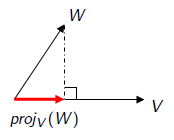
\includegraphics[scale=0.6]{img/bank_vetores/fig01.png}}

Observe que o vetor $\proj_V(W)$ é um múltiplo escalar de $V$. Isto é, existe um número real $\alpha$ tal que $\proj_V(W) = \alpha V$.
Determine este número real $\alpha$ observando que o vetor $W - \proj_V(W)$ é ortogonal a $V$. Demonstre que 

$$\proj_V(W) = \dfrac{\herm{W,V}}{\herm{V,V}}\, V\ .$$
\end{problem}



\begin{solution}
Para resolver este problema você não precisa já ter estudado o conceito de projeção ortogonal. Este exercício pede apenas que uma expressão seja demonstrada. Observe que os passos desta demonstração estão escritos no próprio enunciado.

\medskip
Pela definição de projeção ortogonal, o vetor $\proj_V(W)$ é paralelo ao vetor $V$. Logo existe um número real $\alpha$ tal que $\proj_V(W) = \alpha V$. O vetor diferença $W - \proj_V(W)$ (linha pontilhada da figura) é ortogonal a $V$. Logo o produto escalar entre estes dois vetores é igual a zero.

$$\herm{W - \proj_V(W),V}=0\ \Rightarrow\ \herm{W - \alpha V,V}=0 \ \Rightarrow\ \herm{W,V} - \alpha\herm{V,V}=0\ \Rightarrow$$

$$\alpha\herm{V,V} = \herm{W,V}\ \Rightarrow\alpha = \dfrac{\herm{W,V}}{\herm{V,V}}\ .$$

\medskip
Substituindo este valor de $\alpha$ em $\proj_V(W) = \alpha V$ obtemos

$$\proj_V(W) = \dfrac{\herm{W,V}}{\herm{V,V}}\, V\ .$$

\end{solution}






\begin{problem}
Considere o triângulo de vértices $A=(1,0,1)$, $B=(7,3,4)$ e \linebreak 
$C=(3,-1,4)$. Seja $H$ o pé da altura do triângulo $ABC$ relativa a base $AB$, isto é, seja $H$ o ponto da reta $AB$ de modo que as retas $AB$ e $HC$ são perpendiculares. Use o exercício anterior para determinar as coordenadas do ponto $H$.
\end{problem}

\begin{solution}
\centerline{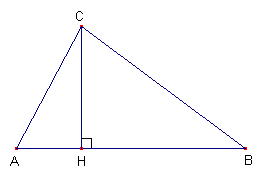
\includegraphics[scale=0.6]{img/bank_vetores/fig09.png}}

O vetor $\overrightarrow{AH}$ é a projeção ortogonal do vetor $\overrightarrow{AC}$ sobre o vetor $\overrightarrow{AB}$. Isto é, 

$$\overrightarrow{AH}\ =\ \proj_{\overrightarrow{AB}}(\overrightarrow{AC})\ =\ \dfrac{\herm{\overrightarrow{AC},\overrightarrow{AB}}}{\herm{\overrightarrow{AB},\overrightarrow{AB}}}\, \overrightarrow{AB}\ .$$

Como $\overrightarrow{AB}=(6,3,3)$ e $\overrightarrow{AC}=(2,-1,3)$ obtemos

$$\overrightarrow{AH}\ =\ \dfrac{12-3+9}{36+9+9}\, (6,3,3)\ =\ \dfrac{1}{3}\, (6,3,3)\ =\ (2,1,1)\ .$$

Como $\overrightarrow{AH}=H-A$, obtemos $H = A + \overrightarrow{AH} = (1,0,1)+(2,1,1)=(3,1,2)$.

Portanto $H=(3,1,2)$. 
\end{solution}

\begin{problem}
Um velho manuscrito descrevia a localização de um tesouro enterrado.

\medskip
{\it ``Há somente duas árvores, $A$ e $B$, em um terreno plano,
e um canteiro de tomates. $A$ é uma mangueira e $B$ uma jaboticabeira. A partir do centro $K$ do canteiro, meça a distância em
linha reta até a mangueira. Vire $90^o$ à esquerda e percorra a mesma distância até o ponto $C$. Volte ao canteiro.
Meça a distância em linha reta até a jaboticabeira. Vire $90^o$ à direita e percorra a mesma distância até o ponto $D$.
O tesouro está no ponto médio $T$ do segmento $CD$.''}

\medskip
Um aventureiro achou o manuscrito, identificou as árvores mas,
como o canteiro \linebreak desaparecera com o passar do tempo, não conseguiu localizá-lo e desistiu do tesouro.
O aluno Sá Bido, nas mesmas condições, diz que seria capaz de localizar o tesouro. Mostre como você resolveria o problema,
isto é, dê as coordenadas de $T$ sabendo que as coordenadas da mangueira e da jaboticabeira são $A=(5,3)$ e $B=(8,2)$.
\end{problem}


\begin{solution}
A figura a seguir ilustra a situação descrita no enunciado.

\centerline{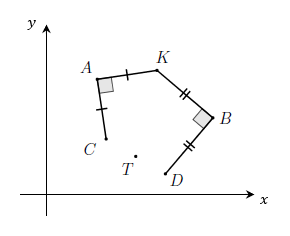
\includegraphics[scale=0.8]{img/bank_vetores/fig16.png}}

Como o aluno Sá Bido afirmou que seria capaz de localizar o tesouro, então a localização do tesouro não pode depender da posição do centro $K$ do canteiro, que é desconhecida. Então vamos considerar que o centro do canteiro está localizado no ponto de coordenadas $K=(a,b)$ em que $a$ e $b$ são números desconhecidos. Se o aluno fez uma afirmação correta, então a localização $T$ do tesouro não pode depender de $a$ e de $b$. Vejamos.

\medskip
Temos que $\overrightarrow{AK} = K - A = (a-5,b-3)$.
Como o vetor $\overrightarrow{AC}$ é obtido do vetor $\overrightarrow{AK}$ por uma rotação de $90^o$ no sentido horário,
sabemos que $\overrightarrow{AC} = (b-3 , -(a-5)) = (b-3 , -a+5)$. Daí
$$C = A + \overrightarrow{AC} = (5,3) + (b-3 , -a+5) = (b+2 , -a+8)$$
Analogamente temos que  $\overrightarrow{BK} = K - B = (a-8,b-2)$.
Como o vetor $\overrightarrow{BD}$ é obtido do vetor $\overrightarrow{BK}$ por uma rotação de $90^o$ no sentido anti-horário,
sabemos que $\overrightarrow{BD} = ( -(b-2) , a-8) = (-b+2 , a-8)$. Daí
$$D = B + \overrightarrow{BD} = (8,2) + (-b+2 , a-8) = (-b+10 , a-6)$$
Como as coordenadas do ponto médio $T$ do segmento $CD$ são a média aritmética das coordenadas de $C$ e de $D$, 
finalmente conseguimos as coordenadas do tesouro

$$T = \dfrac{C+D}{2} = \left( \dfrac{(b+2)+(-b+10)}{2} , \dfrac{(-a+8)+(a-6)}{2} \right) =       
\left(  \dfrac{2+10}{2} , \dfrac{8-6}{2}    \right) = (6,1).$$
\end{solution}


\begin{problem}
A figura é composta por quadrados pequenos iguais dentro de um retângulo de lado horizontal 73 e lado vertical 94.
Calcule o lado de cada quadrado pequeno.
\end{problem}

\begin{solution} 
Introduza na figura um sistema de coordenados como indicado a seguir.
Considere os vetores $V=(a,b)$ e $W=(-b,a)$ ortogonais e de mesma norma também indicados na figura.

\centerline{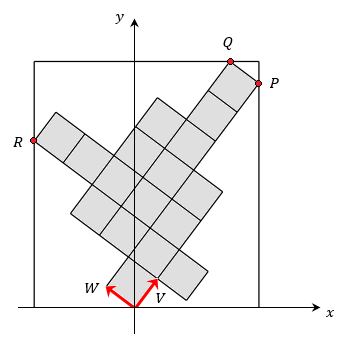
\includegraphics[scale=0.6]{img/bank_vetores/fig15.png}}


As coordenadas dos pontos $P$, $Q$ e $R$ indicados na figura são expressas em termos das coordenadas dos vetores $V$ e $W$ como

$$ P = 7V+W  = (7a-b,7b+a)    $$
$$ Q = 7V+2W = (7a-2b,7b+2a)  $$
$$ R = 2V+5W = (2a-5b,2b+5a)  $$

O lado vertical do retângulo é a coordenada $y$ de $Q$. Daí obtemos $7b+2a=94$.
O lado horizontal do retângulo é a diferença entre a coordenada $x$ de $P$ e a coordenada $x$ de $R$.
Daí obtemos $x_P - x_R = (7a-b) - (2a-5b) = 5a+4b = 73$. Esses duas equações formam o seguinte sistema linear.

$$\left\{ \begin{array}{rrrrr}
 2a & + &  7b &   = & 94 \\
 5a & + &  4b &   = & 73 \end{array} \right.$$

Resolvendo este sistema obtemos $a=5$ e $b=12$.
Como o lado do quadrado pequeno é a norma do vetor $V$ ou a norma do vetor $W$, o lado do quadrado pequeno é

$$\sqrt{a^2 + b^2} = \sqrt{5^2 + 12^2} = \sqrt{25 + 144} = \sqrt{169} = 13.$$
\end{solution} 


